\documentclass [a4paper] {article}
\usepackage[utf8]{inputenc}
\title{Ciencia de datos, práctica 4}
\author{Juan Casado Ballesteros, Samuel García Gonzalez, Iván Anaya Martín}
\usepackage{Sweave}
\begin{document}
\maketitle

\begin{abstract}

\end{abstract}

\newpage
\tableofcontents

\begin{Schunk}
\begin{Sinput}
> plot_kmeans <- function (clusters, centers, xlab="", ylab="") {
+   maxx <- max(clusters[[1]][,1])
+   maxy <- max(clusters[[1]][,2])
+   minx <- min(clusters[[1]][,1])
+   miny <- min(clusters[[1]][,2])
+   for (cluster in clusters){
+     maxx <- max(maxx, max(cluster[,1]))
+     maxy <- max(maxy, max(cluster[,2]))
+     minx <- min(minx, min(cluster[,1]))
+     miny <- min(miny, min(cluster[,2]))
+ 
+   }
+   color_i <- 1
+   colors = c("red", "blue", "pink", "yellow", "black", "brown")
+   for (cluster in clusters){
+     plot(cluster[,1], cluster[,2], type="p", col=colors[color_i],  xlim=c(minx, maxx), ylim=c(miny, maxy), xlab=xlab, ylab=ylab)
+     par(new=TRUE)
+     color_i <- (color_i%%(length(colors)+1))+1
+   }
+   plot(centers[,1], centers[,2],   type="p", col="green", xlim=c(minx, maxx), ylim=c(miny, maxy), xlab=xlab, ylab=ylab)
+ }
> distance <- function (point1, point2) {
+   acc <- 0
+   len <- length(point1)
+   for (i in 1:len){
+     acc <- acc + (point1[i]-point2[i])^2
+   }
+   acc^(1/2)
+ }
> kmeans_cluster <- function (data, centroids) {
+   d_default <- distance(c(max(data), max(data)), c(min(data), min(data)))
+   classification <- c()
+   for (j in 1:nrow(data)){
+       point <- data[j,]
+       best_c <- 0
+       best_d <- d_default
+       for (i in 1:nrow(centroids)){
+         centroid <- centroids[i,]
+         d <- distance (point, centroid)
+         if (d < best_d){
+           best_d <- d
+           best_c <- i
+         }
+     }
+     classification <- c(classification, best_c)
+   }
+   classification <- as.data.frame(classification)
+   rownames(classification) <- rownames(datos1)
+   classification
+ }
> kmeans_split <- function (data, cluster) {
+   clusters=cbind(cluster,data)
+   cluster1=subset(clusters,clusters[,1]==1)
+   cluster2=subset(clusters,clusters[,1]==2)
+   cluster1=cluster1[,-1]
+   cluster2=cluster2[,-1]
+   list(cluster1, cluster2)
+ }
> kmeans_new_centroids <- function(split){
+   centroids <- c()
+   for (cluster in split) {
+     for (colum in cluster) {
+       acc <- 0
+       for (element in colum){
+         acc <- acc + element/length(colum)
+       }
+       centroids <- c(centroids, acc)
+     }
+   }
+   t(matrix(centroids,length(split[[1]]),length(split)))
+ }
> same_centroids <- function(c1, c2){
+   len <- length(c1)
+   ans <- T
+   for (i in 1:len){
+     if (c1[i]!=c2[i]){
+       ans <- F
+     }
+   }
+   ans
+ }
\end{Sinput}
\end{Schunk}

\begin{Schunk}
\begin{Sinput}
> datos1 <- read.table("datos1.txt")
> datos1
\end{Sinput}
\begin{Soutput}
  Teoria Laboratorio
1      4           4
2      3           5
3      1           2
4      5           5
5      0           1
6      2           2
7      4           5
8      2           1
\end{Soutput}
\end{Schunk}

\begin{Schunk}
\begin{Sinput}
> centroides <- matrix(c(0,1,2,2),2,2)
> centroides <- t(centroides)
> centroides
\end{Sinput}
\begin{Soutput}
     [,1] [,2]
[1,]    0    1
[2,]    2    2
\end{Soutput}
\end{Schunk}

\begin{Schunk}
\begin{Sinput}
> classkms<-kmeans(datos1,centroides,4)
\end{Sinput}
\end{Schunk}

\begin{Schunk}
\begin{Sinput}
> classkms$cluster
\end{Sinput}
\begin{Soutput}
1 2 3 4 5 6 7 8 
2 2 1 2 1 1 2 1 
\end{Soutput}
\begin{Sinput}
> classkms$centers
\end{Sinput}
\begin{Soutput}
  Teoria Laboratorio
1   1.25        1.50
2   4.00        4.75
\end{Soutput}
\begin{Sinput}
> classkms$size
\end{Sinput}
\begin{Soutput}
[1] 4 4
\end{Soutput}
\end{Schunk}

\begin{Schunk}
\begin{Sinput}
> classkms$iter
\end{Sinput}
\begin{Soutput}
[1] 1
\end{Soutput}
\begin{Sinput}
> classkms$ifault
\end{Sinput}
\begin{Soutput}
[1] 0
\end{Soutput}
\end{Schunk}

\begin{Schunk}
\begin{Sinput}
> classkms$totss
\end{Sinput}
\begin{Soutput}
[1] 42.75
\end{Soutput}
\begin{Sinput}
> classkms$withinss
\end{Sinput}
\begin{Soutput}
[1] 3.75 2.75
\end{Soutput}
\begin{Sinput}
> classkms$totss.withinss
\end{Sinput}
\begin{Soutput}
NULL
\end{Soutput}
\begin{Sinput}
> classkms$betweenss
\end{Sinput}
\begin{Soutput}
[1] 36.25
\end{Soutput}
\end{Schunk}

\begin{Schunk}
\begin{Sinput}
> clusters <- cbind(classkms$cluster,datos1)
> cluster1 <- subset(clusters,clusters[,1]==1)
> cluster2 <- subset(clusters,clusters[,1]==2)
> cluster1 <- cluster1[,-1]
> cluster2 <- cluster2[,-1]
> clusters <- list(cluster1, cluster2)
\end{Sinput}
\end{Schunk}

\includegraphics{entrega-representacion_del_resultado}

\begin{Schunk}
\begin{Soutput}
     [,1] [,2]
[1,] 1.25 1.50
[2,] 4.00 4.75
\end{Soutput}
\end{Schunk}
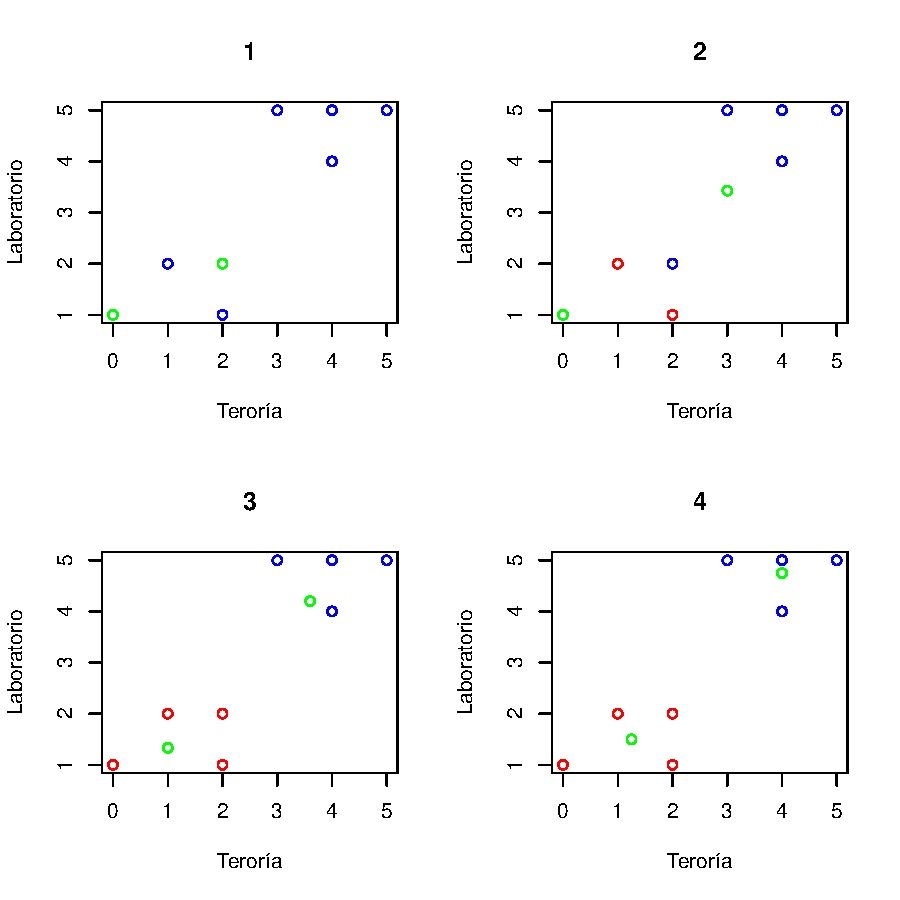
\includegraphics{entrega-custom_kmeans}


\end{document}
